\documentclass{standalone}
\usepackage{tikz}
\usetikzlibrary{patterns, positioning}

\begin{document}
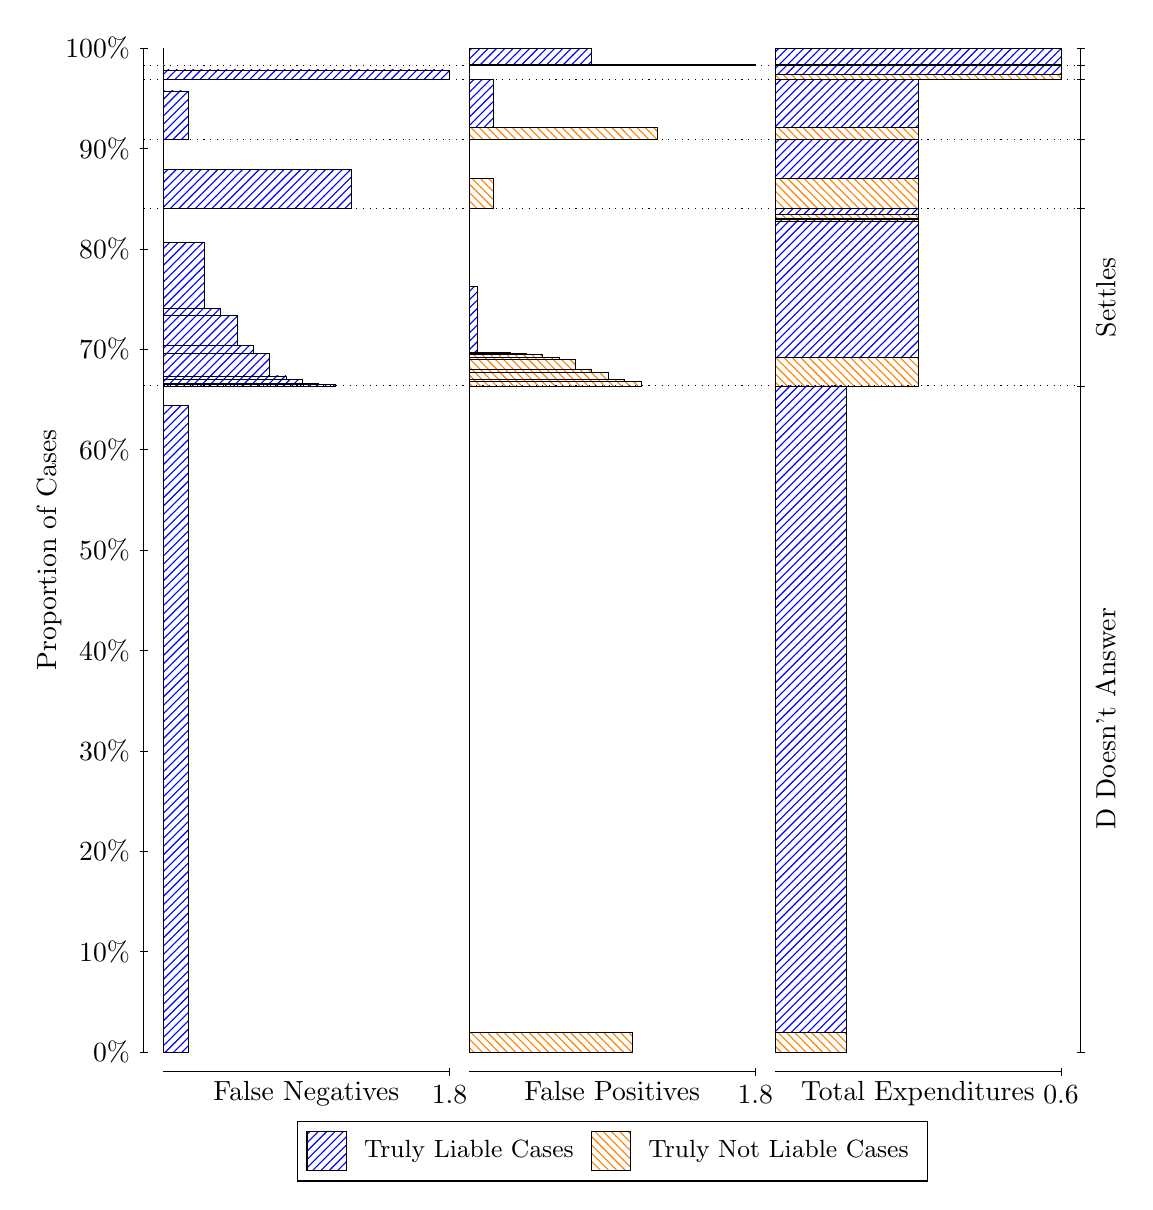
\begin{tikzpicture}
\draw[black, very thin] (1.5,1.75) -- (1.5,14.5);
\node[rotate=90, anchor=center] at (0.3, 8.125) {Proportion of Cases};
\draw[black, very thin] (1.45,1.75) -- (1.55,1.75);
\node[anchor=east] at (1.45, 1.75) {0\%};
\draw[black, very thin] (1.45,3.025) -- (1.55,3.025);
\node[anchor=east] at (1.45, 3.025) {10\%};
\draw[black, very thin] (1.45,4.3) -- (1.55,4.3);
\node[anchor=east] at (1.45, 4.3) {20\%};
\draw[black, very thin] (1.45,5.575) -- (1.55,5.575);
\node[anchor=east] at (1.45, 5.575) {30\%};
\draw[black, very thin] (1.45,6.85) -- (1.55,6.85);
\node[anchor=east] at (1.45, 6.85) {40\%};
\draw[black, very thin] (1.45,8.125) -- (1.55,8.125);
\node[anchor=east] at (1.45, 8.125) {50\%};
\draw[black, very thin] (1.45,9.4) -- (1.55,9.4);
\node[anchor=east] at (1.45, 9.4) {60\%};
\draw[black, very thin] (1.45,10.675) -- (1.55,10.675);
\node[anchor=east] at (1.45, 10.675) {70\%};
\draw[black, very thin] (1.45,11.95) -- (1.55,11.95);
\node[anchor=east] at (1.45, 11.95) {80\%};
\draw[black, very thin] (1.45,13.225) -- (1.55,13.225);
\node[anchor=east] at (1.45, 13.225) {90\%};
\draw[black, very thin] (1.45,14.5) -- (1.55,14.5);
\node[anchor=east] at (1.45, 14.5) {100\%};

\draw[black, very thin] (13.4,1.75) -- (13.4,14.5);
\draw[black, very thin] (13.35,1.75) -- (13.45,1.75);
\node[anchor=west] at (13.35, 1.75) {};
\draw[black, very thin] (13.35,10.21) -- (13.45,10.21);
\node[anchor=west] at (13.35, 10.21) {};
\draw[black, very thin] (13.35,12.46) -- (13.45,12.46);
\node[anchor=west] at (13.35, 12.46) {};
\draw[black, very thin] (13.35,13.343) -- (13.45,13.343);
\node[anchor=west] at (13.35, 13.343) {};
\draw[black, very thin] (13.35,14.104) -- (13.45,14.104);
\node[anchor=west] at (13.35, 14.104) {};
\draw[black, very thin] (13.35,14.28) -- (13.45,14.28);
\node[anchor=west] at (13.35, 14.28) {};
\draw[black, very thin] (13.35,14.5) -- (13.45,14.5);
\node[anchor=west] at (13.35, 14.5) {};

\draw[black, very thin, pattern color=blue, pattern=north east lines] (1.75,1.75) rectangle (2.0614,9.9635);
\draw[black, very thin, pattern color=orange, pattern=north west lines] (1.75,9.9635) rectangle (1.75,10.21);
\draw[black, very thin, pattern color=blue, pattern=north east lines] (1.75,10.21) rectangle (3.93,10.228);
\draw[black, very thin, pattern color=blue, pattern=north east lines] (1.75,10.228) rectangle (3.7224,10.245);
\draw[black, very thin, pattern color=blue, pattern=north east lines] (1.75,10.245) rectangle (3.5148,10.296);
\draw[black, very thin, pattern color=blue, pattern=north east lines] (1.75,10.296) rectangle (3.3071,10.337);
\draw[black, very thin, pattern color=blue, pattern=north east lines] (1.75,10.337) rectangle (3.0995,10.624);
\draw[black, very thin, pattern color=blue, pattern=north east lines] (1.75,10.624) rectangle (2.8919,10.722);
\draw[black, very thin, pattern color=blue, pattern=north east lines] (1.75,10.722) rectangle (2.6843,11.1);
\draw[black, very thin, pattern color=blue, pattern=north east lines] (1.75,11.1) rectangle (2.4767,11.195);
\draw[black, very thin, pattern color=blue, pattern=north east lines] (1.75,11.195) rectangle (2.269,12.033);
\draw[black, very thin, pattern color=orange, pattern=north west lines] (1.75,12.033) rectangle (1.75,12.46);
\draw[black, very thin, pattern color=blue, pattern=north east lines] (1.75,12.46) rectangle (4.1376,12.962);
\draw[black, very thin, pattern color=orange, pattern=north west lines] (1.75,12.962) rectangle (1.75,13.343);
\draw[black, very thin, pattern color=blue, pattern=north east lines] (1.75,13.343) rectangle (2.0614,13.955);
\draw[black, very thin, pattern color=orange, pattern=north west lines] (1.75,13.955) rectangle (1.75,14.104);
\draw[black, very thin, pattern color=blue, pattern=north east lines] (1.75,14.104) rectangle (5.3833,14.222);
\draw[black, very thin, pattern color=orange, pattern=north west lines] (1.75,14.222) rectangle (1.75,14.28);
\draw[black, very thin, pattern color=orange, pattern=north west lines] (1.75,14.28) rectangle (1.75,14.293);
\draw[black, very thin, pattern color=blue, pattern=north east lines] (1.75,14.293) rectangle (1.75,14.5);
\draw[black, very thin, pattern color=orange, pattern=north west lines] (5.6333,1.75) rectangle (7.7095,1.9963);
\draw[black, very thin, pattern color=blue, pattern=north east lines] (5.6333,1.9963) rectangle (5.6333,10.21);
\draw[black, very thin, pattern color=orange, pattern=north west lines] (5.6333,10.21) rectangle (7.8133,10.264);
\draw[black, very thin, pattern color=orange, pattern=north west lines] (5.6333,10.264) rectangle (7.6057,10.288);
\draw[black, very thin, pattern color=orange, pattern=north west lines] (5.6333,10.288) rectangle (7.3981,10.382);
\draw[black, very thin, pattern color=orange, pattern=north west lines] (5.6333,10.382) rectangle (7.1905,10.418);
\draw[black, very thin, pattern color=orange, pattern=north west lines] (5.6333,10.418) rectangle (6.9829,10.55);
\draw[black, very thin, pattern color=orange, pattern=north west lines] (5.6333,10.55) rectangle (6.7752,10.572);
\draw[black, very thin, pattern color=orange, pattern=north west lines] (5.6333,10.572) rectangle (6.7752,10.574);
\draw[black, very thin, pattern color=orange, pattern=north west lines] (5.6333,10.574) rectangle (6.5676,10.61);
\draw[black, very thin, pattern color=orange, pattern=north west lines] (5.6333,10.61) rectangle (6.36,10.622);
\draw[black, very thin, pattern color=orange, pattern=north west lines] (5.6333,10.622) rectangle (6.1524,10.637);
\draw[black, very thin, pattern color=blue, pattern=north east lines] (5.6333,10.637) rectangle (5.7371,11.475);
\draw[black, very thin, pattern color=blue, pattern=north east lines] (5.6333,11.475) rectangle (5.6333,12.46);
\draw[black, very thin, pattern color=orange, pattern=north west lines] (5.6333,12.46) rectangle (5.9448,12.841);
\draw[black, very thin, pattern color=blue, pattern=north east lines] (5.6333,12.841) rectangle (5.6333,13.343);
\draw[black, very thin, pattern color=orange, pattern=north west lines] (5.6333,13.343) rectangle (8.021,13.493);
\draw[black, very thin, pattern color=blue, pattern=north east lines] (5.6333,13.493) rectangle (5.9448,14.104);
\draw[black, very thin, pattern color=orange, pattern=north west lines] (5.6333,14.104) rectangle (5.6333,14.162);
\draw[black, very thin, pattern color=blue, pattern=north east lines] (5.6333,14.162) rectangle (5.6333,14.28);
\draw[black, very thin, pattern color=orange, pattern=north west lines] (5.6333,14.28) rectangle (9.2667,14.293);
\draw[black, very thin, pattern color=blue, pattern=north east lines] (5.6333,14.293) rectangle (7.1905,14.5);
\draw[black, very thin, pattern color=orange, pattern=north west lines] (9.5167,1.75) rectangle (10.425,1.9963);
\draw[black, very thin, pattern color=blue, pattern=north east lines] (9.5167,1.9963) rectangle (10.425,10.21);
\draw[black, very thin, pattern color=orange, pattern=north west lines] (9.5167,10.21) rectangle (11.333,10.572);
\draw[black, very thin, pattern color=blue, pattern=north east lines] (9.5167,10.572) rectangle (11.333,12.304);
\draw[black, very thin, pattern color=orange, pattern=north west lines] (9.5167,12.304) rectangle (11.333,12.319);
\draw[black, very thin, pattern color=blue, pattern=north east lines] (9.5167,12.319) rectangle (11.333,12.337);
\draw[black, very thin, pattern color=orange, pattern=north west lines] (9.5167,12.337) rectangle (11.333,12.387);
\draw[black, very thin, pattern color=blue, pattern=north east lines] (9.5167,12.387) rectangle (11.333,12.46);
\draw[black, very thin, pattern color=orange, pattern=north west lines] (9.5167,12.46) rectangle (11.333,12.841);
\draw[black, very thin, pattern color=blue, pattern=north east lines] (9.5167,12.841) rectangle (11.333,13.343);
\draw[black, very thin, pattern color=orange, pattern=north west lines] (9.5167,13.343) rectangle (11.333,13.493);
\draw[black, very thin, pattern color=blue, pattern=north east lines] (9.5167,13.493) rectangle (11.333,14.104);
\draw[black, very thin, pattern color=orange, pattern=north west lines] (9.5167,14.104) rectangle (13.15,14.162);
\draw[black, very thin, pattern color=blue, pattern=north east lines] (9.5167,14.162) rectangle (13.15,14.28);
\draw[black, very thin, pattern color=orange, pattern=north west lines] (9.5167,14.28) rectangle (13.15,14.293);
\draw[black, very thin, pattern color=blue, pattern=north east lines] (9.5167,14.293) rectangle (13.15,14.5);
\draw[black, dotted] (1.5,10.21) -- (13.4,10.21);
\draw[black, dotted] (1.5,12.46) -- (13.4,12.46);
\draw[black, dotted] (1.5,13.343) -- (13.4,13.343);
\draw[black, dotted] (1.5,14.104) -- (13.4,14.104);
\draw[black, dotted] (1.5,14.28) -- (13.4,14.28);
\draw[black, very thin] (1.75,1.5) -- (5.3833,1.5);
\node[anchor=north] at (3.5667, 1.5) {False Negatives};
\draw[black, very thin] (5.3833,1.45) -- (5.3833,1.55);
\node[anchor=north] at (5.3833, 1.45) {1.8};

\draw[black, very thin] (5.6333,1.5) -- (9.2667,1.5);
\node[anchor=north] at (7.45, 1.5) {False Positives};
\draw[black, very thin] (9.2667,1.45) -- (9.2667,1.55);
\node[anchor=north] at (9.2667, 1.45) {1.8};

\draw[black, very thin] (9.5167,1.5) -- (13.15,1.5);
\node[anchor=north] at (11.333, 1.5) {Total Expenditures};
\draw[black, very thin] (13.15,1.45) -- (13.15,1.55);
\node[anchor=north] at (13.15, 1.45) {0.6};

\node[black, centered, rotate=90] at (13.72, 5.9799) {D Doesn't Answer};
\node[black, centered, rotate=90] at (13.72, 11.335) {Settles};





\draw (7.449999999999999,1.5) node[draw=none] (baseCoordinate) {};
\begin{scope}[align=center]
        \matrix[scale=0.5, draw=black, below=0.5cm of baseCoordinate, nodes={draw}, column sep=0.1cm]{
            \node[rectangle, draw, minimum width=0.5cm, minimum height=0.5cm, pattern=north east lines, pattern color=blue] {}; &
            \node[draw=none, font=\small] (B) {Truly Liable Cases}; &
            \node[rectangle, draw, minimum width=0.5cm, minimum height=0.5cm, pattern=north west lines, pattern color=orange] {}; &
            \node[draw=none, font=\small] (B) {Truly Not Liable Cases}; \\
            };
\end{scope}

\end{tikzpicture}
\end{document}